\documentclass{article}
\usepackage{tabto}
\usepackage{graphicx}
\usepackage{float}
\usepackage{amsmath}
\usepackage{esint}
\usepackage{steinmetz}
\usepackage{hyperref}

\renewcommand{\baselinestretch}{1.25}

\title{Formelblad elektriska kretsar och fält EEM076}
\author{Edvin Alestig}

\begin{document}
\maketitle
\tableofcontents

\newpage
\section{Storheter och enheter}

\textbf{Storhet} \tab \textbf{Enhet}
\\
Effekt (P) \tab Watt (W)
\\
Elektriskt flöde, flux (\(\Phi_E\)) \tab (V \(\cdot\) m)
\\
Elektriskt fält (E) \tab (N/C)
\\
Energi (W) \tab Joule (J)
\\
Frekvens (f) \tab Hertz (Hz)
\\
Impedans (Z) \tab Ohm ($\Omega$)
\\
Induktans (L) \tab Henry (H)
\\
Kapacitans (C) \tab Farad (F)
\\
Konduktivitet (\(\sigma\)) \tab \( ( \Omega \cdot m )^{-1} \)
\\
Kraft (F) \tab Newton (N)
\\
Laddning (Q)  \tab Coloumb (C)
\\
Magnetfält (B) \tab Tesla (T)
\\
Magnetiskt flöde, flux (\(\Phi_B\)) \tab Weber (Wb)
\\
Potentiell energi (U) \tab Joule (J)
\\
Resistans (R) \tab Ohm ($\Omega$)
\\
Resistivitet (\(\rho\)) \tab \(( \Omega \cdot m )\)
\\
Spänning (v) \tab Volt (V)
\\
Ström (I) \tab Ampere (A)
\\
Strömdensitet (J) \tab \((A/m^2)\)
\\
Vinkelhastighet (\(\omega\)) \tab (rad/s)



%% -- %%
\section{Lagar}

\textbf{Ohms lag} \tab  $ v=RI $
\\
\textbf{Effektlagen} \tab  $ P = Iv = RI^2 = \frac{v^2}{R} $
\\
\textbf{Kirchhoffs spänningslag (KVL)} \tab $ \sum v = 0 $  i en loop
\\
\textbf{Kirchhoffs strömlag (KCL)} \tab $ \sum I_{in} = \sum I_{out} $  i en nod
\\
\textbf{Energiprincipen} \tab $ \sum P = 0 $ i en krets
\\
\textbf{Coloumbs lag} \tab \( \vec{F}_{12} = k_e \frac{q_1q_2}{r^2} \hat{r}_{12} \)
\\
\textbf{Gauss lag} \tab \( \vec{\Phi_E} = \oiint \vec{E} \cdot d\vec{A} = \frac{Q}{\varepsilon_0} \)
\\
\textbf{Biot-Savarts lag} \tab \( \vec{B} = \int d\vec{B} = \frac{\mu_0I}{4\pi} \int \frac{d\vec{s} \times \hat{r}}{r^2} \)
\\
\textbf{Amperes lag} \tab \( \oint \vec{B} \cdot d\vec{s} = \mu_0 \cdot I_{enc} \)
\\
\textbf{Faradays lag} \tab \( \vec{\Phi_B} = \iint \vec{B} \cdot d \vec{A} = BA \cos \theta = BA \cos \omega t \)
\\ 
\tab \tab \tab \( \varepsilon = \Delta V = \oint \vec{E} \cdot d \vec{s} = -N \frac{d \Phi_B}{dt} \)
\\
\textbf{Lorentzkraft} \tab \( \vec{F} = q(\vec{E} + \vec{v} \times \vec{B}) \)


%% -- %%

\section{Maxwells ekvationer}
\[ \textrm{Faradays lag: } \oint \vec{E} \cdot d\vec{s} = -\frac{d\Phi_B}{dt} \]
\[ \textrm{Gauss lag (EF): } \Phi_E = \oiint \vec{E} \cdot d\vec{A} = \frac{Q}{\mu_0} \]
\[ \textrm{Gauss lag (MF): } \Phi_B = \oiint \vec{B} \cdot d\vec{A} \]
\[ \textrm{Ampere-Maxwells lag: } \varepsilon = \oint \vec{B} \cdot d\vec{s} = \mu_0 ( I + \varepsilon_0 \frac{d\Phi_E}{dt}) \]

%% -- %%
\section{Konstanter}

Coloumbkonstanten \tab \( k_e = \frac{1}{4 \pi \varepsilon_0} = 8.99 \cdot 10^9 \frac{Nm^2}{C^2} \)
\\
Elektrisk permittivitet i vakuum \tab \( \varepsilon_0 = \frac{10^{-9}}{36 \pi} \)
\\
Elementarladdningen \tab \( e = 1.602 \cdot 10^{-19} \) C
\\
Tomrummets permeabilitet \tab \( \mu_0 = 4\pi \cdot 10^{-7} \) H/m (Tm/A)
\\
Ljusets hastighet i vakuum \tab \( c = 299~792~458 \) m/s

%% -- %%
 \newpage
\section{Formler}
\subsection{Kretsar}
\[ I(t) = \frac{dq(t)}{dt} \]

\[ Q(t) = \int_{t_0}^t I(t) \cdot dt + Q(t_0) \]

\[ W = \int_{t_1}^{t_2} P(t) \cdot dt \]

\subsubsection{I kondensatorer}
\[ Q = Cv \]
\[ I = \frac{dQ}{dt} = C \frac{dv}{dt} \]
\[ P = IV = Cv \frac{dv}{dt} \]
\[ W = \int_{t_0}^t P(t) \cdot dt = \int_{t_0}^t Cv \frac{dv}{dt} = C \int_{v(t_0)}^{v(t)} v \cdot dv = \frac{C}{2}(v(t)^2 - v(t_0)^2) \]
\[ W = \frac{Cv^2}{2}, v(t_0) = 0 \]
\[ v(t) = \frac{1}{C} \int_{t_0}^t I(t)\cdot dt + v(t_0) \]
\[ C = \varepsilon_0 \frac{A}{d} = \frac{Q}{|Ed|} \]
\[ U = \frac{1}{2} \varepsilon_0 E^2Ad = \frac{1}{2} C V^2 \textrm{ (Potentiell energi)} \]

\subsubsection{I induktorer}
\[ v = L \frac{dI}{dt} \]
\[ W = \frac{LI^2}{2}, I(t_0) = 0 \]
\[ I(t) = \frac{1}{L} \int_{t_0}^t v(t) \cdot dt + I(t_0) \]
\[ P = IV = LI \frac{di}{dt} \]
\[ \textrm{Self-inductance: } \varepsilon_L = -N \frac{d\Phi_B}{dt} = L \frac{dI}{dt} \]
\[ L = \frac{N \Phi_B}{I} = \frac{\mu_0 N^2 A}{l} \]
\[ U = \frac{1}{2} LI^2 \]
The power, or rate at which an external emf works to overcome self-induced emf and pass current: \[ P_L = \frac{dW_{ext}}{dt} = IL\frac{dI}{dt} \]

\subsection{Elektriska fält}
\[ \vec{E} = k_e \frac{q}{r^2} \hat{r}_{12} \]
\[ \vec{F}_E  = q \vec{E} \]
\[ \vec{E}_{total} = \sum \vec{E}_i \textrm{ (diskreta laddningar)} \]
\[ \vec{E}_{total} = \int_{L1}^{L2} \vec{E}_l \cdot dl \textrm{ (kontinuerliga laddningar)} \]

\subsubsection{Flytta laddningar}
\[ W =\int_R^{\infty} \vec{F} \cdot d\vec{r} = \frac{-k_eq_1q_2}{R} \textrm{ (utanför fält)} \]
\[ W = -qE_0r \]

\subsubsection{Dipoler}
\[ \vec{P} = q \vec{d} \]
\[ \vec{\tau} = \vec{p} \times \vec{E} \]
\[ \tau = p \cdot E \cdot \sin{\theta} \]
\[ U = Ep(\sin \theta_1 - \sin \theta_0) \]

\subsubsection{Elektriskt flöde (flux)}
\[ \vec{\Phi} = \sum \vec{E}_i \]
\[ \vec{\Phi} = \int_{L1}^{L2} \vec{E}_l \cdot d\vec{l} \]
\[ \vec{\Phi} = \iint \vec{E}\hat{n} \cdot d\vec{A} = \iint \vec{E} \cdot d\vec{A} \cdot \cos{\theta} \textrm{ i två dimensioner}\]

\subsubsection{Elektrisk potential}
\[ \frac{W}{q} = -\int_A^B \vec{E} \cdot d\vec{r} = -Ed = \Delta V \]
\[ \vec{E} = -\frac{dV}{d\vec{r}} = -\nabla v  = -grad(v) \textrm{ (typ flerdimensionell derivata)} \]

\subsubsection{Ström, konduktivitet \& resitivitet}
\[ I = \iint \vec{J} \cdot d\vec{A} = \frac{dQ}{A \cdot dt} \]
\[ \vec{J} = \sigma \vec{E} \]
\[ J = \sigma E = \sigma \frac{\Delta V}{l} = \frac{I}{A} \textrm{ (uniform field)} \]
\[ \Delta V = \frac{l}{\sigma}J = \frac{l}{\sigma A} I = RI \]
\[ \rho = \frac{1}{\sigma} \]
\[ \rho = \rho_0 [1 + \alpha (T - T_0)] \textrm{ när det beror på temperatur} \]

\subsubsection{Magnetfält, generatorer, motorer och induktion}
\[ \vec{B} = \frac{\mu_0 I}{4\pi} \int \frac{d \vec{s} \times \hat{r}}{r^2} \implies B = \frac{\mu_0 I}{2\pi r} \textrm{ i en oändlig wire} \]
\[ B = \frac{\mu_0 NI}{l} = \mu_0 nI \textrm{ i en oändlig solenoid} \]
\[ I = \frac{|\varepsilon|}{R} = \frac{NBA\omega}{R} \sin \omega t \]
\[ P = \frac{(NBA\omega)^2}{R} \sin^2 \omega t\]
Total work done by external source to increase current from 0 to I in a magnetic field/inductor: \[ W_{ext} = U_B = \int_0^I LI \cdot dI  = \frac{1}{2}LI^2 \]

\subsubsection{Elektromagnetiska vågor}
\[ c = \lambda f = \frac{\omega}{k} = \frac{E}{B} \]
\[ \vec{E} = E_y(x, t) \hat{j} = E_0 \cos(kx-\omega t) \hat{j} \]
\[ \vec{B} = B_z(x, t( \hat{k} = B_0 \cos(kx-\omega t) \hat{k} \]
\[ \frac{\partial E_y}{\partial x} = -\frac{\partial  B_z}{\partial t} \]
\[ \frac{\partial E_y}{\partial x}  = -kE_0 \sin(kx - \omega t) \]
\[ \frac{\partial B_z}{\partial t} = \omega B_0 \sin(kx-\omega t) \]

\subsection{Växelström}
\subsubsection{Grundläggande}
\[ v(t) = V_m \cos(\omega t + \theta) \]
\[ \omega = 2 \pi f \]
\[ \sin(z) = \cos(z - 90^\circ) \]
\[ V_{rms} = \frac{V_m}{\sqrt{2}} \]
\[ I_{rms} = \frac{I_m}{\sqrt{2}} \]
\[ P_{avg} = V_{rms} \cdot I_{rms} = \frac{V^2_{rms}}{R} = I^2_{rms} R \]
\[ v(t) = V_m \cos(\omega t + \theta) \leftrightarrow V = V_m \phase{\theta} \]

\subsubsection{Notation}
\[ z = x + jy = |z|(\cos \theta + j \sin \theta) = |z| \phase{\theta} = |z| e^{j \theta} \]
\[ z = r \phase{\theta} \rightarrow z = r( \cos \theta + j \cdot \sin \theta ) \]
\[ z = x + jy \rightarrow z = \sqrt{x^2 + y^2} \phase{ \tan^{-1} \frac{y}{x} } \]
\[ (b \phase{c})(d \phase{e}) = bd \phase{c+e} \]
\[ \frac{b \phase{c}}{d \phase{e}} = \frac{b}{d} \phase{c-e} \]

\subsubsection{Induktorer}
\[ V_L = V_m \phase{\theta} \]
\[ I_L = I_m \phase{\theta - \frac{\pi}{2}} \]

\subsubsection{Kondensatorer}
\[ V_L = V_m \phase{\theta} \]
\[ I_L = I_m \phase{\theta + \frac{\pi}{2}} \]

\subsubsection{Tids-/frekvensdomäner}
\[ \textrm{Över en resistor: } v = Ri \leftrightarrow V = RI \]
\[ \textrm{Över en induktor: } v = L \frac{di}{dt} \leftrightarrow V = j \omega LI \]
\[ \textrm{Över en kondensator: } v = \frac{1}{C} \int i \cdot dt \leftrightarrow V = \frac{1}{j \omega C}I \]

\subsubsection{Impedans}
\[ Z = \frac{V}{I} \Leftrightarrow V = IZ \]
\[ Z_R = R, \quad Z_L = j \omega L = \omega L \phase{\frac{\pi}{2}}, \quad Z_C = \frac{1}{j \omega C} = \frac{1}{\omega C} \phase{-\frac{\pi}{2}} \]
\[ \textrm{Reaktans } = Im(Z), \quad \textrm{Resistans } = Re(Z) \]

\subsubsection{Resonans}
\[ f_0 = \frac{1}{2\pi \sqrt{LC}} \rightarrow Im(Z) = 0 \]
\[ \textrm{Kvalitetsfaktor } Q_s = \frac{2\pi f_0 L}{R} = \frac{1}{2\pi f_0 CR} \]
\[ Z_s = R \left[1 + j Q_s \left( \frac{f}{f_0} - \frac{f_0}{f} \right) \right] \]

\subsection{Effekt i växelström}

\subsubsection{Resistive load (\(\theta = 0 \))}
\[ v(t) = V_m \cos(\omega t), \quad i(t) = I_m \cos(\omega t) \]
\[ P(t) = V_m I_m \cos^2(\omega t) \]
\[ P_{avg} = \frac{V_m I_m}{2} = V_{rms} \cdot I_{rms} \]

\subsubsection{Inductive load (\(z = \omega L \phase{90^\circ} \))}
\[ v(t) = V_m \cos(\omega t), \quad i(t) = I_m \cos(\omega t - 90^\circ) = I_m \sin(\omega t) \]
\[ P(t) = \frac{V_m I_m}{2} \sin{2\omega t} \]
\[ P_{avg} = 0 \]

\subsubsection{Capacitive load (\(z = \frac{1}{\omega C} \phase{-90^\circ} \))}
\[ v(t) = V_m \cos(\omega t), \quad i(t) = I_m\cos(\omega t + 90^\circ) = -I_m \sin(\omega t) \]
\[ P(t) = -\frac{V_m I_m}{2} \sin(2 \omega t) \]
\[ P_{avg} = 0 \] 

\subsubsection{Effekttyper}
\[ \textrm{Real power: } P = V_{rms} I_{rms} \cos(\theta_v - \phi_i) \]
\[ \textrm{Reactive power: } Q = V_{rms} I_{rms}\sin(\theta_v - \phi_i) \quad \textrm{ (enhet: VAR)}\]
\[ \textrm{Complex power: } S = P + jQ = V_{rms}I_{rms}\phase{\theta_v - \phi_i} \quad \textrm{ (enhet: VA)} \]
\[ \textrm{Apparent power: } |S| = V_{rms}I_{rms} \quad \textrm{ (enhet: VA)} \]

\subsubsection{Power factor}
\[ PF = \frac{P}{|S|} = \cos(\theta_v - \phi_i) \leq 1 \]
\[ \textrm{Power angle: } \theta_v - \phi_i \]

\subsection{Amplifier}
\[ \textrm{Voltage gain: } A_v = \frac{V_o}{V_i} \]
\[ \textrm{Current gain: } A_i = \frac{i_o}{i_i} = A_v \frac{R_i}{R_L} \]

\subsubsection{Operational amplifier (op-amp)}
\[ \textrm{Common mode signal: } V_{cm} = \frac{1}{2}(V_1 + V_2) \]
\[ \textrm{Differential signal: } V_d = V_1 - V_2 \]

\begin{figure}[H]
    \centering
        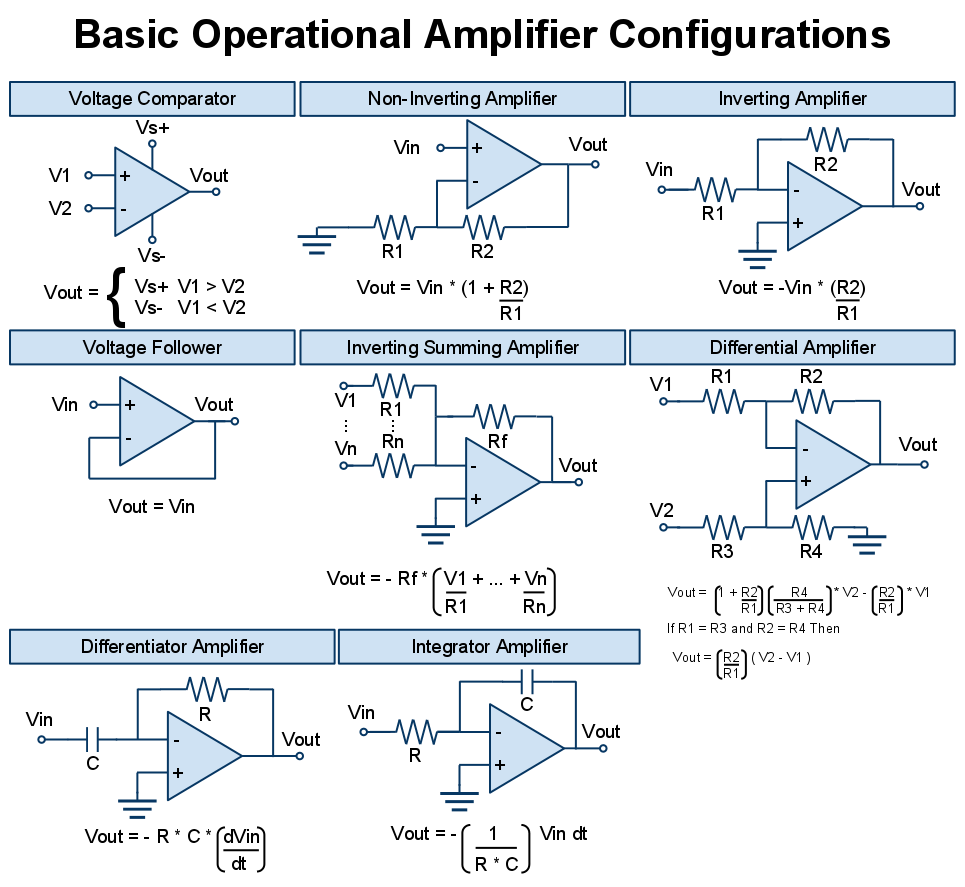
\includegraphics[scale=0.35]{opamps.png}
    \label{fig:opamps}
\end{figure}

\subsubsection{Transfer frequency}
\[ H(f) = \frac{V_{out}}{V_{in}} \]
\[ \textrm{Decibel dB } = 20 \log_{10}(|H(f)|) \]
\[ \textrm{Butterworth transfer function } H(f) = \frac{H_0}{\sqrt{1 + \left( \frac{f}{f_B} \right)^{2n}}} \]
\[ f_B = \textrm{ break frequency }, H_0 = H(0) = \textrm{ DC gain} \]


%% -- %%
\section{Ekvivalenta kretsar}
\subsection{Seriekoppling}

Resistans $ R_{eq} = \sum R_n $
\\
Kapacitans  $ C_ {eq} = (\sum C_n ^{-1})^{-1} $ \tab (\( C_{eq} = \frac{C_1C_2}{C_1+C_2} \) vid endast 2 kondensatorer)
\\
Induktans $ L_{eq} = \sum L_n $
\\
Impedans \( Z_{eq} = \sum Z_n \)
\\ \\
Spänningsdelning \tab $ v_{n} = R_nI = \frac{R_n}{R_{eq}} \cdot v_{total} $

\subsection{Parallellkoppling}

Resistans $ R_{eq} = (\sum R_n^{-1})^{-1} $ \tab ($ R_{eq} = \frac{R_1R_2}{R_1 + R_2} $ vid endast 2 resistorer)
\\
Kapacitans $ C_{eq} = \sum C_n $
\\
Induktans $ L_{eq} = (\sum L_n^{-1})^{-1} $ \tab (\(L_{eq} = \frac{L_1L_2}{L_1+L_2}\) vid endast 2 induktorer)
\\
Impedans \( Z_{eq} = (\sum Z_n^{-1})^{-1} \) \tab (\( Z_{eq} = \frac{Z_1Z_2}{Z_1 + Z_2} \) vid endast 2 impedanser)
\\ \\
Strömdelning \tab $ I_1 = \frac{R_2}{R_1+R_2} \cdot I_{total} \quad I_2 = \frac{R_1}{R_1+R_2} \cdot I_{total} $

\subsection{Thévenin equivalent circuit (behöver förbättras)}

\begin{figure}[H]
    \centering
        \includegraphics[scale=0.5]{thevenin.png}
    \label{fig:thevenin}
\end{figure}

\begin{enumerate}
    \item Disconnect the load \(R_L\) and replace with an open circuit.
    \item Find the open circuit voltage \(V_{oc}\).
    \item Find the equivalent resistance \(R_{eq}\) of the network with all independent sources turned off.
    \item \(v_{th} = v_{oc}\) and \(R_{th} = R_{eq}\).
\end{enumerate}

\subsection{Norton equivalent circuit (behöver förbättras)}

\begin{figure}[H]
    \centering
        \includegraphics[scale=0.5]{norton.png}
    \label{fig:norton}
\end{figure}

\begin{enumerate}
    \item Replace the load \(R_L\) with a short circuit.
    \item Find the short circuit current \(I_{sc}\).
    \item Find the equivalent resistance \(R_{eq}\) of the network with all independent sources turned off.
    \item \(I_N = I_{sc}\) and \(R_N = R_{eq}\).
\end{enumerate}

\subsection{Source transformation - Thévenin and Norton}
\(R_{th} = R_N = R_{eq}\) and \(v_{th} = I_NR_{eq}\)
\\
Genom att kombinera Thévenin och Norton kan man kraftigt förenkla en delkrets.


%% -- %%
\section{Verktyg och metoder}
\subsection{Kretsar}
\subsubsection*{Node voltage analysis}
Analysera spänningsskillnader gentemot en referensnod (jord eller den nod med flest kopplingar). Lös med ekvationssystem.

\begin{enumerate}
	\item Välj en referensnod och sätt den till 0 V.
	\item Sätt variabler för varje nod.
	\item Applicera KCL på varje nod.
	\item Räkna ut spänningen genom att räkna ut spänningsdifferensen mellan två noder.
\end{enumerate}

Tips: Räkna $ I_{out} $ som positiv i varje resistor. 

\subsubsection*{Supernod}
Spänningskälla som ej är direkt kopplad till referensnoden kan göras om till en supernod. Nodens spänning är källans spänning och båda ändars kopplingar räknas som supernodens kopplingar.

\subsubsection*{Mesh current analysis}
Analysera loopar i en krets (medsols). Applicera KVL på varje loop. Lös med ekvationssystem.

\subsubsection*{Supermesh}
Strömkälla i kretsen. Kombinera loopar in i en större superloop. $ I_{super} = I_1 - I_2 $

\subsubsection*{Superposition}
Går endast att applicera på linjära kretsar med flera ström- och/eller spänningskällor. Varje källa kan analyseras separat för att sedan läggas ihop.
\begin{enumerate}
	\item Stäng av alla källor förutom en.
	\begin{itemize}
		\item v = 0 blir en kortsluten krets.
		\item I = 0 blir en öppen krets.
		\item Räkna ut källans kretspåverkan.
	\end{itemize}
	\item Lägg ihop alla källors påverkan.
\end{enumerate}




\end{document}